\documentclass[tikz,border=0pt]{standalone}
\usepackage{xcolor}
\usetikzlibrary{calc}
% Palette: Sam_Comm_final.png by eye, and the drones and raiders.
\definecolor{ink}{HTML}{3B2340}
\definecolor{sky}{HTML}{EFC46A}
\definecolor{skyhi}{HTML}{F5DA92}
\definecolor{skylow}{HTML}{E9B060}
\definecolor{cloud}{HTML}{F2D58A}
\definecolor{paper}{HTML}{FBEFD0}
\definecolor{cream}{HTML}{FFF6E0}
\definecolor{white}{HTML}{FFFFFF}
\definecolor{wallA}{HTML}{E88A73}
\definecolor{wallB}{HTML}{EE9F7E}
\definecolor{wallC}{HTML}{E47A7E}
\definecolor{wallD}{HTML}{F0B07E}
\definecolor{wallE}{HTML}{D9765F}
\definecolor{wallF}{HTML}{E99A8A}
\definecolor{greenA}{HTML}{8DBB7E}
\definecolor{greenB}{HTML}{6FA77A}
\definecolor{greenC}{HTML}{A9C97F}
\definecolor{greenD}{HTML}{5E9C6A}
\definecolor{greenE}{HTML}{4A8060}
\definecolor{sage}{HTML}{9DB98A}
\definecolor{sagedark}{HTML}{6F8F66}
\definecolor{sagelight}{HTML}{C2D6A6}
\definecolor{window}{HTML}{F6E7A0}
\definecolor{windark}{HTML}{8C5A64}
\definecolor{metal}{HTML}{8D9A93}
\definecolor{metaldark}{HTML}{5E6B66}
\definecolor{metallight}{HTML}{B9C4BC}
\definecolor{wood}{HTML}{B9835A}
\definecolor{wooddark}{HTML}{8C5A3C}
\definecolor{woodlight}{HTML}{D9A66F}
\definecolor{stone}{HTML}{E7C9A0}
\definecolor{stonedark}{HTML}{C9A47E}
\definecolor{concrete}{HTML}{D8C3A4}
\definecolor{concretedark}{HTML}{B8A084}
\definecolor{asphalt}{HTML}{8E7A86}
\definecolor{asphaltdark}{HTML}{6E5C68}
\definecolor{roadline}{HTML}{F6E7A0}
\definecolor{kerb}{HTML}{D8B48C}
\definecolor{red}{HTML}{E0483E}
\definecolor{redlight}{HTML}{F27A6A}
\definecolor{gold}{HTML}{FFB000}
\definecolor{goldlight}{HTML}{FFD54F}
\definecolor{teal}{HTML}{4FA3A0}
\definecolor{tealdark}{HTML}{3C8582}
\definecolor{magenta}{HTML}{FF2E88}
\definecolor{cyan}{HTML}{13CFE3}
\definecolor{violet}{HTML}{8A5BD6}
\definecolor{orange}{HTML}{F2803A}
\definecolor{pink}{HTML}{F48FB1}
\definecolor{glow}{HTML}{4FE6E0}
\definecolor{glowhi}{HTML}{C8FFF9}
\definecolor{hot}{HTML}{FF6A1A}
\definecolor{hothi}{HTML}{FFD07A}
\definecolor{armour}{HTML}{7E7A86}
\definecolor{armourdark}{HTML}{5A5466}
\definecolor{armourlight}{HTML}{A8A2B0}
\definecolor{wasp}{HTML}{E0A82E}
\definecolor{waspdark}{HTML}{B07E1A}
\definecolor{moth}{HTML}{F2E6C8}
\definecolor{mothdark}{HTML}{D2C09A}
\definecolor{hornet}{HTML}{3C8582}
\definecolor{hornetdark}{HTML}{2C6260}
\definecolor{warden}{HTML}{E47A7E}
\definecolor{wardendark}{HTML}{B85A62}
\definecolor{tick}{HTML}{8DBB7E}
\definecolor{tickdark}{HTML}{5E8A5A}
\definecolor{strider}{HTML}{D9765F}
\definecolor{striderdark}{HTML}{A8543F}
\definecolor{jacket}{HTML}{6FA77A}
\definecolor{jacketb}{HTML}{4FA3A0}
\definecolor{jacketc}{HTML}{E88A73}
\definecolor{jacketd}{HTML}{F0B07E}
\definecolor{skin}{HTML}{F2C49A}
\definecolor{skinb}{HTML}{C98C6A}
\definecolor{skinc}{HTML}{8C5A3C}
\definecolor{hair}{HTML}{3B2340}
\definecolor{goo}{HTML}{B6E35A}
\definecolor{goodark}{HTML}{7FB23A}
\newcommand{\Ink}{1.6pt}
\tikzset{inked/.style={draw=ink, line width=\Ink, line join=round, line cap=round}}
\begin{document}
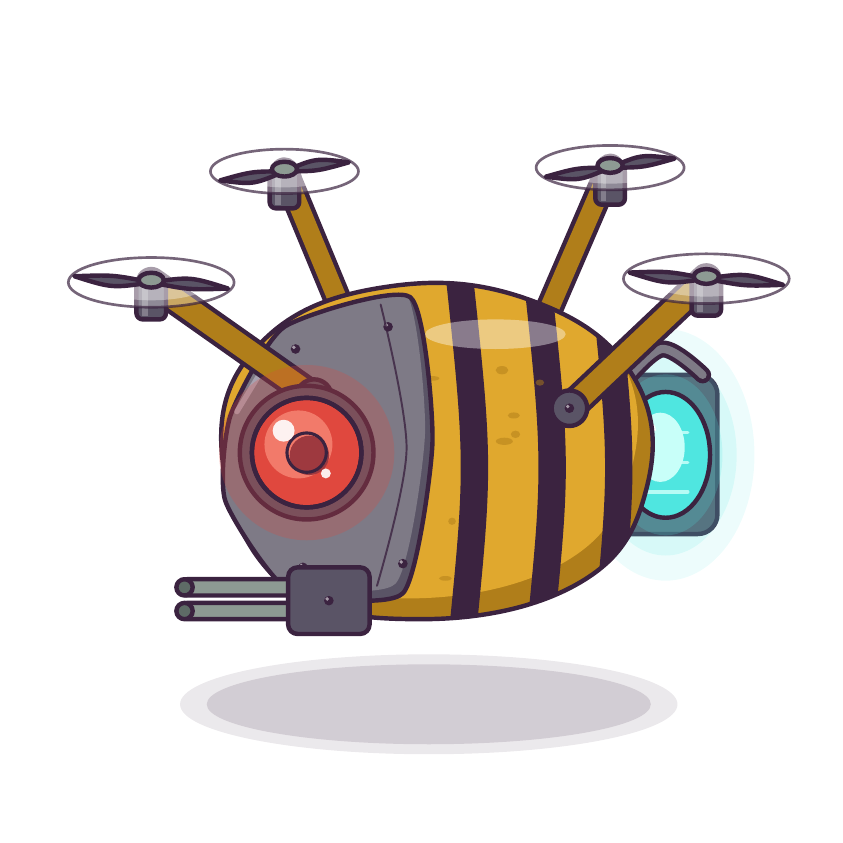
\begin{tikzpicture}
\clip (0,0) rectangle (10,10);
\begin{scope}[shift={(0.3,-0.05)}, scale=0.94]
\fill[ink, opacity=0.10] (5.1,1.55) ellipse (3.36 and 0.675);
\fill[ink, opacity=0.14] (5.1,1.55) ellipse (3 and 0.54);
\draw[ink, line width=10.154pt, line cap=round, line join=round] plot[smooth, tension=0.55] coordinates {(4,6.7) (3.15,8.75)};
\draw[waspdark, line width=6.954pt, line cap=round, line join=round] plot[smooth, tension=0.55] coordinates {(4,6.7) (3.15,8.75)};
\filldraw[inked,fill=armourdark,rounded corners=0.08cm] (2.95,8.25) rectangle (3.35,8.77);
\fill[white, opacity=0.25] (3.02,8.3) rectangle (3.1,8.71);
\filldraw[ink, line width=0.96pt, fill=white, fill opacity=0.32, draw opacity=0.7] (3.15,8.75) ellipse (1 and 0.3);
\fill[white, opacity=0.35] (3.15,8.75) ellipse (0.72 and 0.216);
\filldraw[inked,fill=armourdark] (3.15,8.75) .. controls (3.568,8.93) .. (4.02,8.872) .. controls (3.593,8.751) .. (3.15,8.75) -- cycle;
\filldraw[inked,fill=armourdark] (3.15,8.75) .. controls (2.732,8.57) .. (2.28,8.628) .. controls (2.707,8.749) .. (3.15,8.75) -- cycle;
\filldraw[inked,fill=metal] (3.15,8.78) ellipse (0.17 and 0.1);
\draw[ink, line width=10.154pt, line cap=round, line join=round] plot[smooth, tension=0.55] coordinates {(6.6,6.6) (7.55,8.8)};
\draw[waspdark, line width=6.954pt, line cap=round, line join=round] plot[smooth, tension=0.55] coordinates {(6.6,6.6) (7.55,8.8)};
\filldraw[inked,fill=armourdark,rounded corners=0.08cm] (7.35,8.3) rectangle (7.75,8.82);
\fill[white, opacity=0.25] (7.42,8.35) rectangle (7.5,8.76);
\filldraw[ink, line width=0.96pt, fill=white, fill opacity=0.32, draw opacity=0.7] (7.55,8.8) ellipse (1 and 0.3);
\fill[white, opacity=0.35] (7.55,8.8) ellipse (0.72 and 0.216);
\filldraw[inked,fill=armourdark] (7.55,8.8) .. controls (7.968,8.98) .. (8.42,8.922) .. controls (7.993,8.801) .. (7.55,8.8) -- cycle;
\filldraw[inked,fill=armourdark] (7.55,8.8) .. controls (7.132,8.62) .. (6.68,8.678) .. controls (7.107,8.799) .. (7.55,8.8) -- cycle;
\filldraw[inked,fill=metal] (7.55,8.83) ellipse (0.17 and 0.1);
\filldraw[inked,fill=armourdark,rounded corners=0.25cm] (7.45,3.85) rectangle (9,6);
\fill[glow, opacity=0.1] (8.3,4.92) ellipse (1.2 and 1.7);
\fill[glow, opacity=0.14] (8.3,4.92) ellipse (0.96 and 1.36);
\fill[glow, opacity=0.2] (8.3,4.92) ellipse (0.768 and 1.088);
\filldraw[inked,fill=glow] (8.3,4.92) ellipse (0.6 and 0.85);
\fill[glowhi]  (8.228,5.022) ellipse (0.33 and 0.468);
\fill[white, opacity=0.9] (8.06,5.26) circle (0.108);
\draw[glowhi, opacity=0.85, line width=1.2pt, line cap=round] (8.05,4.42) -- (8.6,4.42);
\draw[glowhi, opacity=0.85, line width=1.2pt, line cap=round] (8.05,4.82) -- (8.6,4.82);
\draw[glowhi, opacity=0.85, line width=1.2pt, line cap=round] (8.05,5.22) -- (8.6,5.22);
\draw[ink, line width=6.142pt, line cap=round, line join=round] plot[smooth, tension=0.55] coordinates {(7.7,5.85) (8.25,6.35) (8.8,6)};
\draw[armour, line width=2.942pt, line cap=round, line join=round] plot[smooth, tension=0.55] coordinates {(7.7,5.85) (8.25,6.35) (8.8,6)};
\fill[waspdark] plot[smooth cycle, tension=0.7] coordinates {(2.3,5) (2.9,6.5) (4.6,7.2) (6.5,7) (7.85,6) (8.05,4.5) (7.15,3.2) (5,2.7) (3.1,3.2)};
\begin{scope}\clip plot[smooth cycle, tension=0.7] coordinates {(2.3,5) (2.9,6.5) (4.6,7.2) (6.5,7) (7.85,6) (8.05,4.5) (7.15,3.2) (5,2.7) (3.1,3.2)};
\begin{scope}[shift={(-0.2,0.28)}]\fill[wasp] plot[smooth cycle, tension=0.7] coordinates {(2.3,5) (2.9,6.5) (4.6,7.2) (6.5,7) (7.85,6) (8.05,4.5) (7.15,3.2) (5,2.7) (3.1,3.2)};\end{scope}
\fill[ink] (5.35,2.3) .. controls (5.6,4.8) .. (5.3,7.6) -- (5.67,7.6) .. controls (5.97,4.8) .. (5.72,2.3) -- cycle;
\fill[ink] (6.4,2.3) .. controls (6.65,4.8) .. (6.35,7.6) -- (6.72,7.6) .. controls (7.02,4.8) .. (6.77,2.3) -- cycle;
\fill[ink] (7.3,2.3) .. controls (7.55,4.8) .. (7.25,7.6) -- (7.62,7.6) .. controls (7.92,4.8) .. (7.67,2.3) -- cycle;
\begin{scope}\clip plot[smooth cycle, tension=0.7] coordinates {(2.3,5) (2.9,6.5) (4.6,7.2) (6.5,7) (7.85,6) (8.05,4.5) (7.15,3.2) (5,2.7) (3.1,3.2)};
\fill[waspdark, opacity=0.5] (6.121,5.103) ellipse (0.115 and 0.049);
\fill[waspdark, opacity=0.5] (6.271,5.197) ellipse (0.063 and 0.05);
\fill[waspdark, opacity=0.5] (6.601,5.896) ellipse (0.057 and 0.042);
\fill[waspdark, opacity=0.5] (5.145,5.953) ellipse (0.099 and 0.032);
\fill[waspdark, opacity=0.5] (7.552,6.48) ellipse (0.096 and 0.055);
\fill[waspdark, opacity=0.5] (5.325,3.251) ellipse (0.087 and 0.032);
\fill[waspdark, opacity=0.5] (5.414,4.023) ellipse (0.052 and 0.049);
\fill[waspdark, opacity=0.5] (6.089,6.064) ellipse (0.086 and 0.056);
\fill[waspdark, opacity=0.5] (6.249,5.452) ellipse (0.082 and 0.041);
\end{scope}
\fill[white, opacity=0.4] (6,6.55) ellipse (0.95 and 0.2);
\end{scope}
\draw[inked] plot[smooth cycle, tension=0.7] coordinates {(2.3,5) (2.9,6.5) (4.6,7.2) (6.5,7) (7.85,6) (8.05,4.5) (7.15,3.2) (5,2.7) (3.1,3.2)};
\fill[armourdark] plot[smooth cycle, tension=0.35] coordinates {(2.42,5.45) (3.15,6.65) (4.85,7.05) (5.15,5.1) (4.75,3.05) (3.2,3.1) (2.35,4.3)};
\begin{scope}\clip plot[smooth cycle, tension=0.35] coordinates {(2.42,5.45) (3.15,6.65) (4.85,7.05) (5.15,5.1) (4.75,3.05) (3.2,3.1) (2.35,4.3)};
\begin{scope}[shift={(-0.1,0.13)}]\fill[armour] plot[smooth cycle, tension=0.35] coordinates {(2.42,5.45) (3.15,6.65) (4.85,7.05) (5.15,5.1) (4.75,3.05) (3.2,3.1) (2.35,4.3)};\end{scope}
\end{scope}
\draw[inked] plot[smooth cycle, tension=0.35] coordinates {(2.42,5.45) (3.15,6.65) (4.85,7.05) (5.15,5.1) (4.75,3.05) (3.2,3.1) (2.35,4.3)};
\draw[armourlight, line width=1.92pt, line cap=round] (2.508,5.504) -- (2.967,6.26);
\fill[ink] (3.3,6.35) circle (0.065);
\fill[white, opacity=0.55] (3.277,6.373) circle (0.026);
\fill[ink] (4.55,6.65) circle (0.065);
\fill[white, opacity=0.55] (4.527,6.673) circle (0.026);
\fill[ink] (4.75,3.45) circle (0.065);
\fill[white, opacity=0.55] (4.727,3.473) circle (0.026);
\fill[ink] (3.4,3.4) circle (0.065);
\fill[white, opacity=0.55] (3.377,3.423) circle (0.026);
\draw[ink, line width=0.7pt, line cap=round, line join=round, opacity=0.8] plot[smooth, tension=0.5] coordinates {(4.45,6.95) (4.8,5) (4.4,3.15)};
\draw[ink, line width=11.224pt, line cap=round, line join=round] plot[smooth, tension=0.55] coordinates {(3.55,5.7) (1.35,7.25)};
\draw[waspdark, line width=8.024pt, line cap=round, line join=round] plot[smooth, tension=0.55] coordinates {(3.55,5.7) (1.35,7.25)};
\filldraw[inked,fill=armourdark] (3.55,5.7) circle (0.24);
\fill[ink] (3.55,5.7) circle (0.065);
\fill[white, opacity=0.55] (3.527,5.723) circle (0.026);
\draw[ink, line width=11.224pt, line cap=round, line join=round] plot[smooth, tension=0.55] coordinates {(7,5.55) (8.85,7.3)};
\draw[waspdark, line width=8.024pt, line cap=round, line join=round] plot[smooth, tension=0.55] coordinates {(7,5.55) (8.85,7.3)};
\filldraw[inked,fill=armourdark] (7,5.55) circle (0.24);
\fill[ink] (7,5.55) circle (0.065);
\fill[white, opacity=0.55] (6.977,5.573) circle (0.026);
\filldraw[inked,fill=metal,rounded corners=0.08cm] (1.75,2.7) rectangle (3.6,2.92);
\filldraw[inked,fill=metaldark] (1.8,2.81) circle (0.11);
\filldraw[inked,fill=metal,rounded corners=0.08cm] (1.75,3.02) rectangle (3.6,3.24);
\filldraw[inked,fill=metaldark] (1.8,3.13) circle (0.11);
\filldraw[inked,fill=armourdark,rounded corners=0.12cm] (3.2,2.5) rectangle (4.3,3.4);
\fill[ink] (3.75,2.95) circle (0.065);
\fill[white, opacity=0.55] (3.727,2.973) circle (0.026);
\filldraw[inked,fill=armourdark] (3.45,4.95) circle (0.903);
\fill[red, opacity=0.25] (3.45,4.95) circle (1.184);
\filldraw[inked,fill=red] (3.45,4.95) circle (0.74);
\fill[redlight] (3.339,5.061) circle (0.459);
\fill[red!60!ink] (3.487,4.913) circle (0.266);
\draw[ink, line width=1.12pt] (3.45,4.95) circle (0.266);
\fill[white, opacity=0.9] (3.139,5.246) circle (0.148);
\fill[white, opacity=0.9] (3.709,4.669) circle (0.067);
\draw[inked] (3.45,4.95) circle (0.74);
\filldraw[inked,fill=armourdark,rounded corners=0.08cm] (1.15,6.75) rectangle (1.55,7.27);
\fill[white, opacity=0.25] (1.22,6.8) rectangle (1.3,7.21);
\filldraw[ink, line width=0.96pt, fill=white, fill opacity=0.32, draw opacity=0.7] (1.35,7.25) ellipse (1.12 and 0.336);
\fill[white, opacity=0.35] (1.35,7.25) ellipse (0.806 and 0.242);
\filldraw[inked,fill=armourdark] (1.35,7.25) .. controls (1.879,7.328) .. (2.389,7.167) .. controls (1.864,7.148) .. (1.35,7.25) -- cycle;
\filldraw[inked,fill=armourdark] (1.35,7.25) .. controls (0.821,7.172) .. (0.311,7.333) .. controls (0.836,7.352) .. (1.35,7.25) -- cycle;
\filldraw[inked,fill=metal] (1.35,7.28) ellipse (0.17 and 0.1);
\filldraw[inked,fill=armourdark,rounded corners=0.08cm] (8.65,6.8) rectangle (9.05,7.32);
\fill[white, opacity=0.25] (8.72,6.85) rectangle (8.8,7.26);
\filldraw[ink, line width=0.96pt, fill=white, fill opacity=0.32, draw opacity=0.7] (8.85,7.3) ellipse (1.12 and 0.336);
\fill[white, opacity=0.35] (8.85,7.3) ellipse (0.806 and 0.242);
\filldraw[inked,fill=armourdark] (8.85,7.3) .. controls (9.379,7.378) .. (9.889,7.217) .. controls (9.364,7.198) .. (8.85,7.3) -- cycle;
\filldraw[inked,fill=armourdark] (8.85,7.3) .. controls (8.321,7.222) .. (7.811,7.383) .. controls (8.336,7.402) .. (8.85,7.3) -- cycle;
\filldraw[inked,fill=metal] (8.85,7.33) ellipse (0.17 and 0.1);
\end{scope}
\end{tikzpicture}
\end{document}
